% Source: AESP_466_ClassWork/Exams/Midterm/figures/mission_geometry.tex
\documentclass[tikz,border=5pt]{standalone}
\usepackage{xcolor}
\usetikzlibrary{arrows.meta}
\definecolor{Garnet}{HTML}{73000A}
\definecolor{USC_Rose}{HTML}{CC2E40}
\definecolor{USC_Blue}{HTML}{466A9F}
\definecolor{USC_Olive}{HTML}{65780B}
\definecolor{USC_Black90}{HTML}{565656}
\definecolor{USC_Black10}{HTML}{ECECEC}
\begin{document}
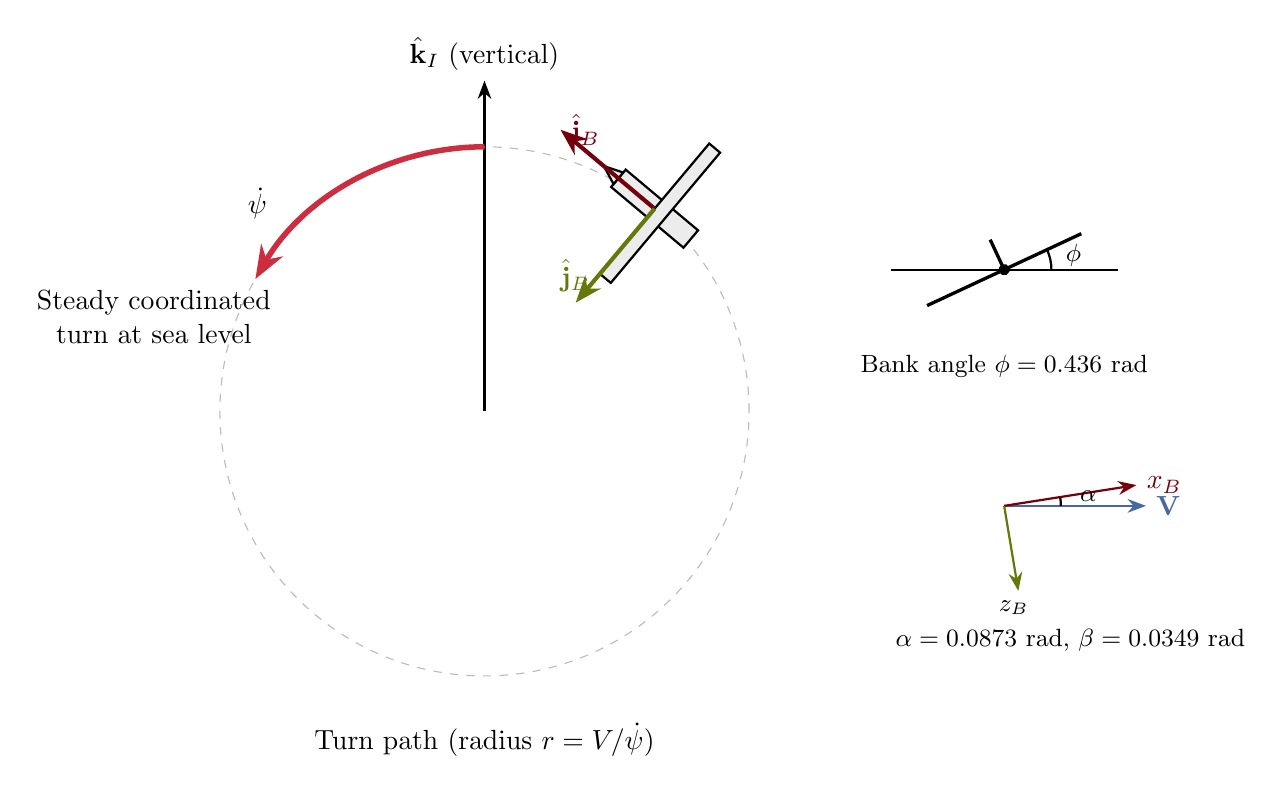
\begin{tikzpicture}[scale=1.2, >=Stealth]
    % Vertical axis
    \draw[->, thick, black] (0,0) -- (0,3.5) node[above] {$\hat{\mathbf{k}}_I$ (vertical)};

    % Turn path circle
    \draw[dashed, USC_Black90!40] (0,0) circle (2.8);
    \node[black, below] at (0,-3.2) {Turn path (radius $r = V/\dot\psi$)};

    % Turn rate arrow
    \draw[->, line width=2pt, USC_Rose] (0,2.8) arc (90:150:2.8);
    \node[black, left] at (-2.2,2.2) {$\dot\psi$};

    % Text annotation
    \node[align=center, black] at (-3.5,1) {Steady coordinated\\turn at sea level};

    % Aircraft position on circle
    \coordinate (aircraft) at (50:2.8);

    % Aircraft body (top view)
    \begin{scope}[shift={(aircraft)}, rotate=-40]
        % Fuselage
        \draw[thick, black, fill=USC_Black10] (-0.5,-0.12) rectangle (0.5,0.12);
        % Wings
        \draw[thick, black, fill=USC_Black10] (0,-0.9) rectangle (0.15,0.9);
        % Tail
        \draw[thick, black, fill=USC_Black10] (-0.5,-0.08) -- (-0.7,0) -- (-0.5,0.08) -- cycle;
    \end{scope}

    % Body axes from aircraft
    \begin{scope}[shift={(aircraft)}, rotate=140]
        \draw[->, line width=1.5pt, Garnet] (0,0) -- (1.3,0) node[right] {$\hat{\mathbf{i}}_B$};
        \draw[->, line width=1.5pt, USC_Olive] (0,0) -- (0,1.3) node[above] {$\hat{\mathbf{j}}_B$};
    \end{scope}

    % Bank angle inset (right side)
    \begin{scope}[shift={(5.5,1.5)}]
        % Horizon line
        \draw[thick, black] (-1.2,0) -- (1.2,0);
        % Banked aircraft (rear view)
        \draw[very thick, black, rotate=25] (-0.9,0) -- (0.9,0);
        \draw[very thick, black, rotate=25] (0,0) -- (0,0.35);
        \fill[black, rotate=25] (0,0) circle (0.06);
        % Bank angle arc
        \draw[thick, black] (0.5,0) arc (0:25:0.5);
        \node[black, right, font=\small] at (0.55,0.15) {$\phi$};
        \node[black, below, font=\small] at (0,-0.8) {Bank angle $\phi = 0.436$ rad};
    \end{scope}

    % Velocity and angle of attack inset (right side, below bank)
    \begin{scope}[shift={(5.5,-1.0)}]
        \draw[->, thick, USC_Blue] (0,0) -- (1.5,0) node[right] {$\mathbf{V}$};
        \draw[->, thick, Garnet] (0,0) -- (1.4,0.22) node[right] {$x_B$};
        \draw[thick] (0.6,0) arc (0:8.5:0.6);
        \node[right, font=\small] at (0.7,0.1) {$\alpha$};
        \draw[->, thick, USC_Olive] (0,0) -- (0.15,-0.9) node[below] {};
        \node[below, font=\small] at (0.1,-0.9) {$z_B$};
        \node[black, below, font=\small] at (0.7,-1.2) {$\alpha = 0.0873$ rad, $\beta = 0.0349$ rad};
    \end{scope}

\end{tikzpicture}
\end{document}
